\documentclass{scrartcl}
% Skapalón frá Hlyni Arnórssyni
% Physics Version 0.2 - 10.Jan 2020
% ---------- Blaðsíðustillingar ---------- 
\usepackage{geometry}

\geometry{
	paper=a4paper, % letterpaper lika til
	top=2.5cm, % Top margin
	bottom=1cm, % Bottom margin
	left=2.5cm, % Left margin
	right=2.4cm, % Right margin
	headheight=0.75cm, % Header height
	footskip=1.5cm, % Space from the bottom margin to the baseline of the footer
	headsep=0.75cm, % Space from the top margin to the baseline of the header
	%showframe, % Uncomment to show how the type block is set on the page
}

% ---------- Íslenska ---------- 
\usepackage[T1]{fontenc}
\usepackage[utf8]{inputenc}
\usepackage[icelandic]{babel}

% ---------- Stærðfræðipakkar frá AMS ---------- 

% \usepackage{amsmath, amsfonts, amsthm, amssymb} % Stærðfræðipakkar

% ---------- Listar/ númeringar ---------- 
\usepackage{enumitem, multicol}

% ---------- Fyrir innsetningu mynda ---------- 
\usepackage{graphicx, float} 
\usepackage{caption}
\newcommand{\source}[1]{\caption*{Source: {#1}} }
\graphicspath{ {./images/} }

%%%%%%%%%%%%%%%%%%%%%%%%%% Hyperlink References %%%%%%%%%%%%%%%%%%%%%%%%%%%
\usepackage{hyperref}


%%%%%%%%%%%%%%%%%%%%%%%%% Code blocks %%%%%%%%%%%%%%%%%%%%%%%%%%%%%%%%%%%%%
\usepackage{listings} %code extracts
%\usepackage{xcolor} %custom colours
\usepackage{mdframed} %nice frames
\usepackage{pgffor} % for loops
\usepackage[table,xcdraw]{xcolor}
\usepackage{float}
\usepackage{multicol, caption}
%support for figures in multicol environment
\newenvironment{Figure}
  {\par\medskip\noindent\minipage{\linewidth}}
  {\endminipage\par\medskip}

% ---------- Skrá fyrir myndir ---------- 
\graphicspath{{graphics/}{Graphics/}{./}}

\begin{document}

%% --- Titil síða / Title page --- %%
\begin{titlepage}
	\centering
	
\includegraphics[width=0.3\textwidth]{ru-logo.eps}\par\vspace{1cm} %<-- RU Logo
	{\scshape\LARGE Reykjavík University\par} %<-- Nafn háskólans (Háskólinn í Reykjavík / Reykjavik University)
	\vspace{1cm}
	{\scshape\Large Verklegt námskeið II\par} %<-- Áfanga titill / Class or course title
	\vspace{1.5cm}
	{\huge\bfseries Requirement Analysis Report\par} %<-- Titill Skýrslu / Title of Report
	{\Large\itshape  Group 2 \par}
	\vspace{2cm}
	{\Large\itshape Helgi Hákonarson}\par %<-- Nafn nemanda / Name of student
	\texttt{helgihak20@ru.is}\par %<-- t-póstfang / e-mail
	\vspace{0.5cm}
	{\Large\itshape Konráð Elí Sigurgeirsson}\par %<-- Nafn nemanda / Name of student
	\texttt{konrad21@ru.is}\par %<-- t-póstfang / e-mail
	\vspace{0.5cm}
	{\Large\itshape Patrekur Þór Agnarsson}\par %<-- Nafn nemanda / Name of student
	\texttt{patrekur20@ru.is}\par %<-- t-póstfang / e-mail
	\vspace{0.5cm}
	{\Large\itshape Sigurður Baldvin Friðriksson}\par %<-- Nafn nemanda / Name of student
	\texttt{sigurdurf21@ru.is}\par %<-- t-póstfang / e-mail
	\vfill
	Teacher\par %<-- (Umsjón höfðu / supervised by)
	Arnar Leifsson%<-- Nafn kennara og aðstoðarkennara í tilraun / Name of Lab Teacher and TA
	\vfill

% Bottom of the page
	{\large \today\par}
\end{titlepage}

% Efnisyfirlit
\tableofcontents
\newpage

%% --- Titil síða endar / Title page ends --- %%

\section{Introduction}
FireSale! is an online marketplace that wants to connect users with each other. Our goal is to simply the process of buying and selling goods and services between users. FireSale! will allow sellers to post items for sale or put on auction. Buyers will be able to buy posted items and bid on auction items. Our focus is that transactions between sellers and buys be as smooth as possible and we strive to create a platform that allows for that.\\


\noindent Our inspiration for FireSale! is based on Craigslist, a large platform where users offer services or products for sale. And bland.is, a local Icelandic web-hub similar to Craigslist but the differences lie in the emphasis on product visibility for bland.is compared to category visibility for Craigslist.\\

\noindent In this document you will find information regarding the requirements for FireSale!, interviews for our requirement analysis, use-cases, user-groups and a wireframe. Some of the data will be located in supplementary files as their format would be ill-fitted for the report.\\

\noindent All of these data points will be important for the first initial design of FireSale!.


\section{List of requirements}

\section{Use cases / scenarios}

\section{User groups and analysis}
% Please add the following required packages to your document preamble:
% \usepackage[table,xcdraw]{xcolor}
% If you use beamer only pass "xcolor=table" option, i.e. \documentclass[xcolor=table]{beamer}
\begin{tabular}{|p{2.5cm}|p{2.5cm}|p{2.5cm}|p{2.5cm}|p{2.5cm}|}
\hline
\rowcolor[HTML]{93C47D} 
\textbf{Name   of the user group} & & & & \\
\rowcolor[HTML]{D9D9D9} 
\textbf{WHO: background} & Buyer & Seller & Buyer / Seller & Browser \\ \hline
Age & 29-36 & 26-36 & 24 - 36 & 18 - 22 \\ \hline
Gender & M / F & M / F & M / F & M / F \\ \hline
Education & Some college & Secondary education - College graduate & Secondary education - Some college & Some College\\ \hline
General computer skills & Intermediate & Expert & Intermediate & Intermediate \\\hline
Number of users (estimates) & 33,33\% & 16,67\% & 41,67\% & 8,33\% \\ \hline
\rowcolor[HTML]{D9D9D9}
\textbf{WHY: Why would the users want to use the software?} & Want the best prices and easily locate what they want to buy & Want their products to be visible to buyers and to easily setup a sale for their   products & Want to easily get rid of their items and find what they want quickly & Want to easily view specific products that peak their interest \\ \hline
\rowcolor[HTML]{D9D9D9} 
\textbf{WHAT: Technical environment} & Web browser / Mobile phone & Web browser / Mobile phone & Web   browser / Mobile phone & Web browser / Mobile phone \\ \hline
\rowcolor[HTML]{D9D9D9} 
\textbf{WHERE: The usage environment} & At home & At home & At home & At home \\ \hline
\rowcolor[HTML]{D9D9D9} 
\textbf{WHEN:Usage of the software} & Monitors pricing and new listings in the categories they are   interested in & Monitors offers and products similar to their offerings & A mix of   buyer and Seller & Browsing new listings and checking category view for their relevant categories \\ \hline
How often & Somewhat often 1-5 times a week every few weeks & Very often 1-3 times a day & Often 1-5   times a week & Seldom 1-5 times a month \\ \hline
For how long & 10 - 60 minutes a week & 30 - 90 minutes a day & 10 - 90 minutes a week & 5-60   minutes a month \\ \hline
User skills & Basic - Intermediate & Expert & Intermediate - Expert & Basic - Intermediate \\ \hline
\rowcolor[HTML]{93C47D} 
\textbf{HOW: Important is this user group?} & Very important & Very important & Some importance & Unimportant \\\hline
\end{tabular}


\section{Wireframes and prototype interviews}

\section{Benchmarking}
There are several key parts of the website that we found would benefit from benchmarking. These sections include the landing page, product page and the search results.\\

These pages are very important for the user experience but are also well defined in the online commerce space. 
\subsection{Landing page}
For the landing page, we take a look at Craigslist and Bland.is.
These websites are those we will draw large inspirations from and it is important to view their differences closely. \textit{See figures 1 and 2}

\begin{Figure}
    \begin{center}
        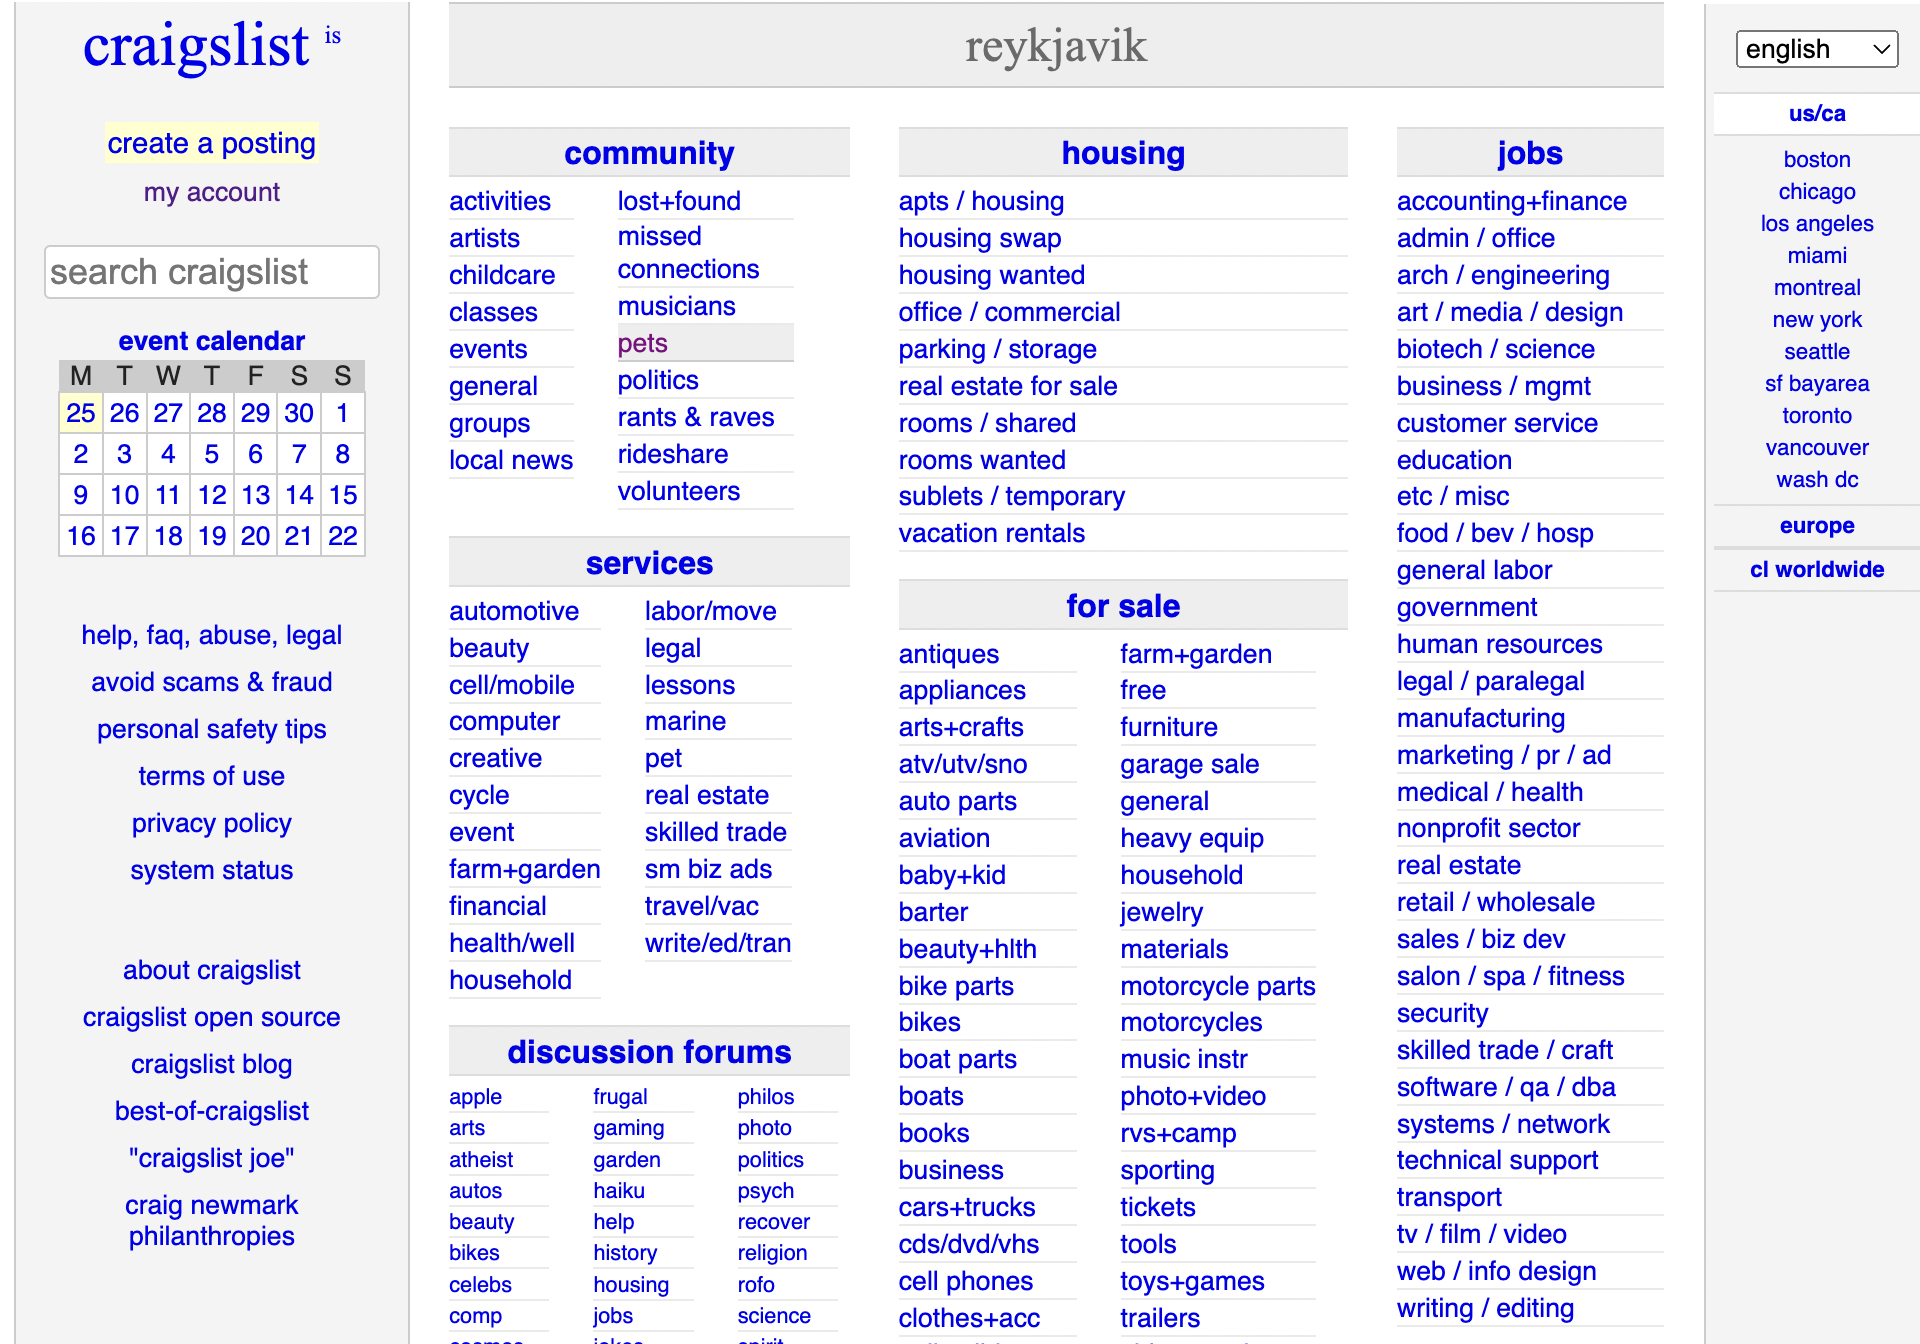
\includegraphics[width=150mm, height=80mm]{Images/benchmarking/landing_page_cl.png}
\captionof{figure}{Craigslist Landing page}
    \end{center}
\end{Figure}
\begin{Figure}
    \begin{center}
        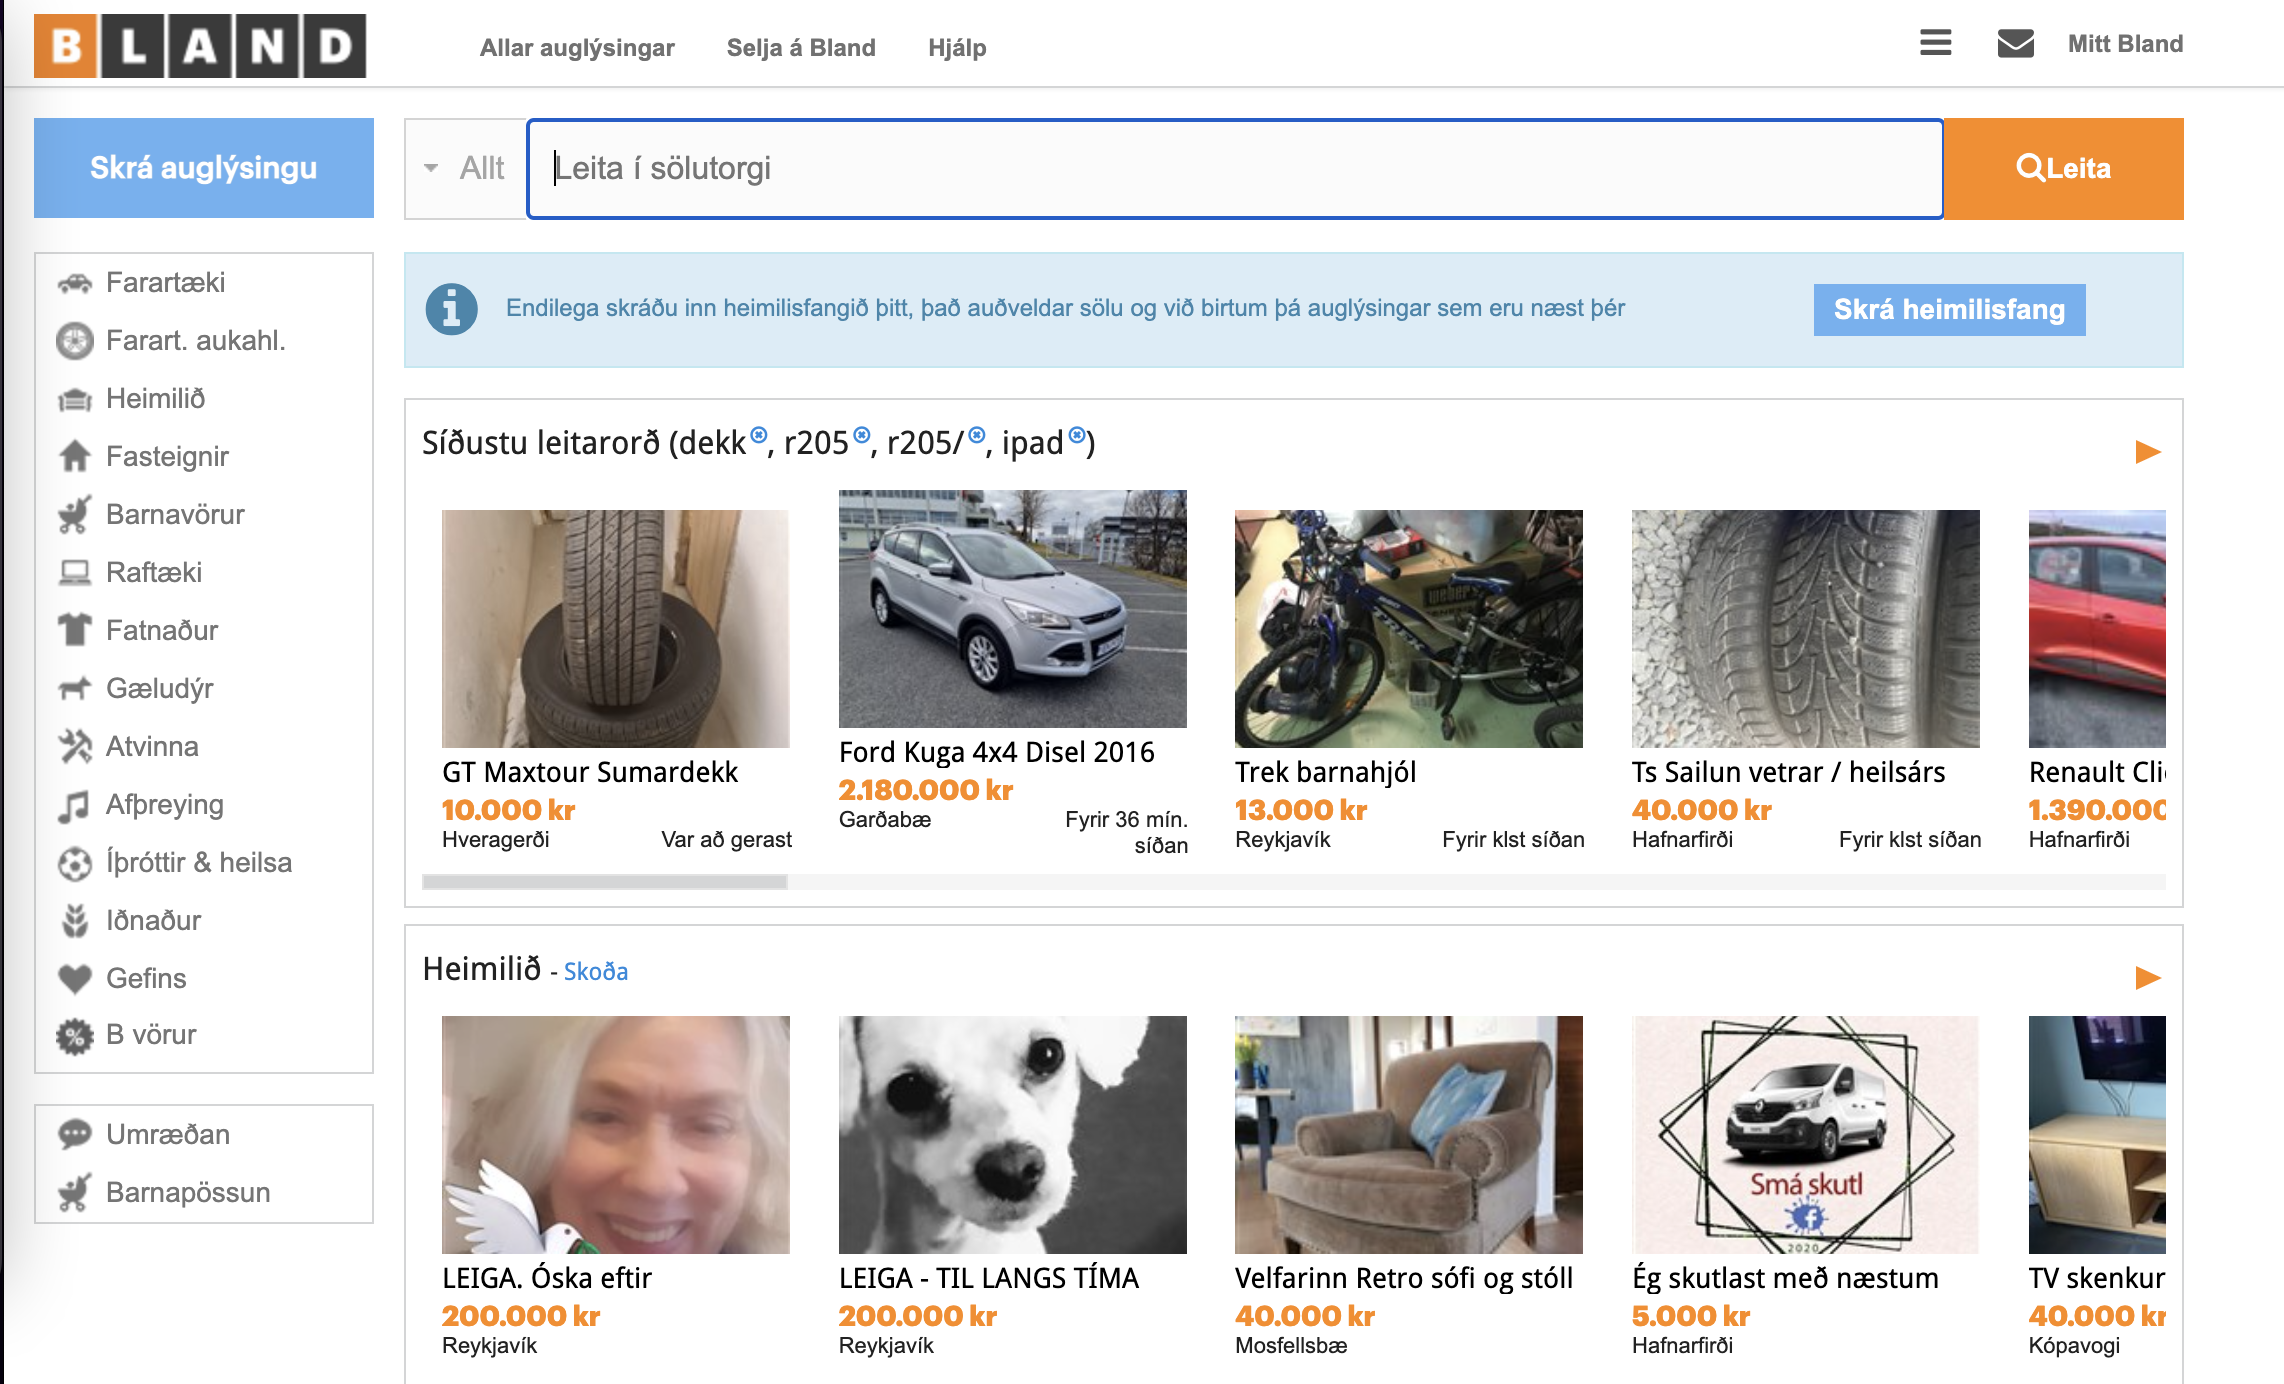
\includegraphics[width=150mm, height=80mm]{Images/benchmarking/landing_page_bland.png}
\captionof{figure}{bland.is Landing page}
    \end{center}
\end{Figure}

Right of the bat, we notice that Craigslist focuses on access to categories and sub-categories whilst bland puts their focus on showing you relevant products you might want to view, utilizing the users recent searches to achieve that.
The search bar is prominent for Bland but for Craigslist, it sort of hides in the UI, rather placing the users' focus on navigating through the categories first. 

\subsection{Product page}
The product page is the last step for the user before checkout. Therefor, important that if the product page sells the user on the product, the checkout process can begin, which is our goal. 

For the product page to be able to sell the user on the product, the most relevant information needs to be clearly visible on their first look. We continue to use Bland and Craigslist for our benchmark, with the edition of a product page from Elko's website. \textit{See figures 3, 4, 5}
\begin{Figure}
    \begin{center}
        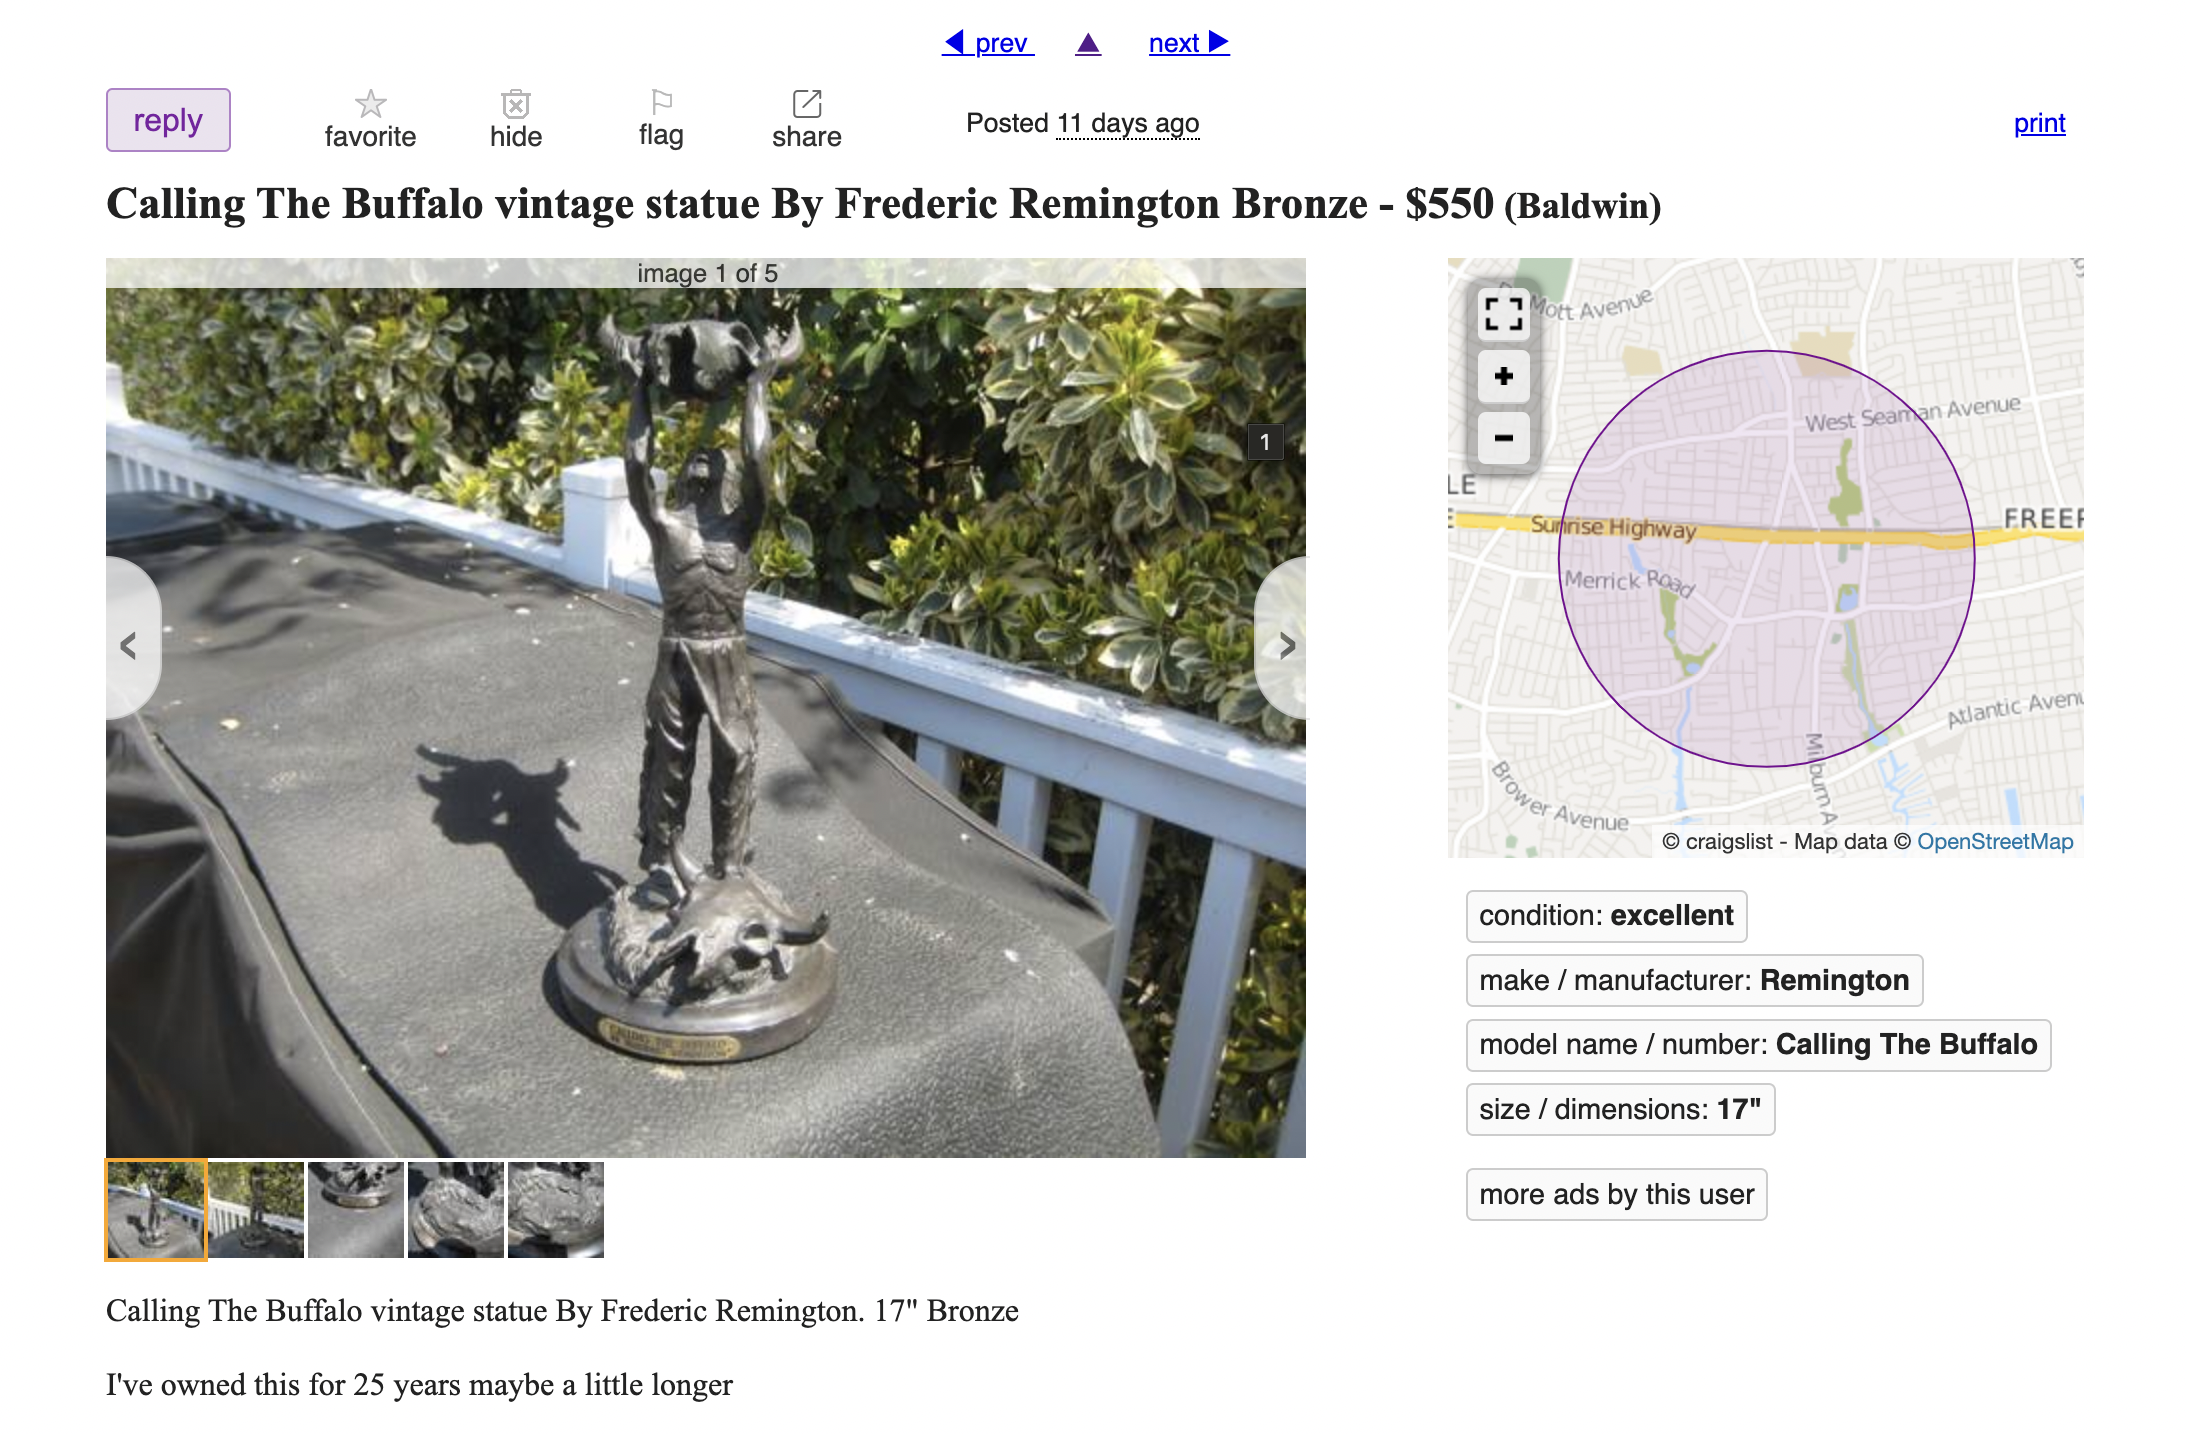
\includegraphics[width=150mm, height=80mm]{Images/benchmarking/product_page_cl.png}
\captionof{figure}{Craigslist Product page}
    \end{center}
\end{Figure}
\begin{Figure}
    \begin{center}
        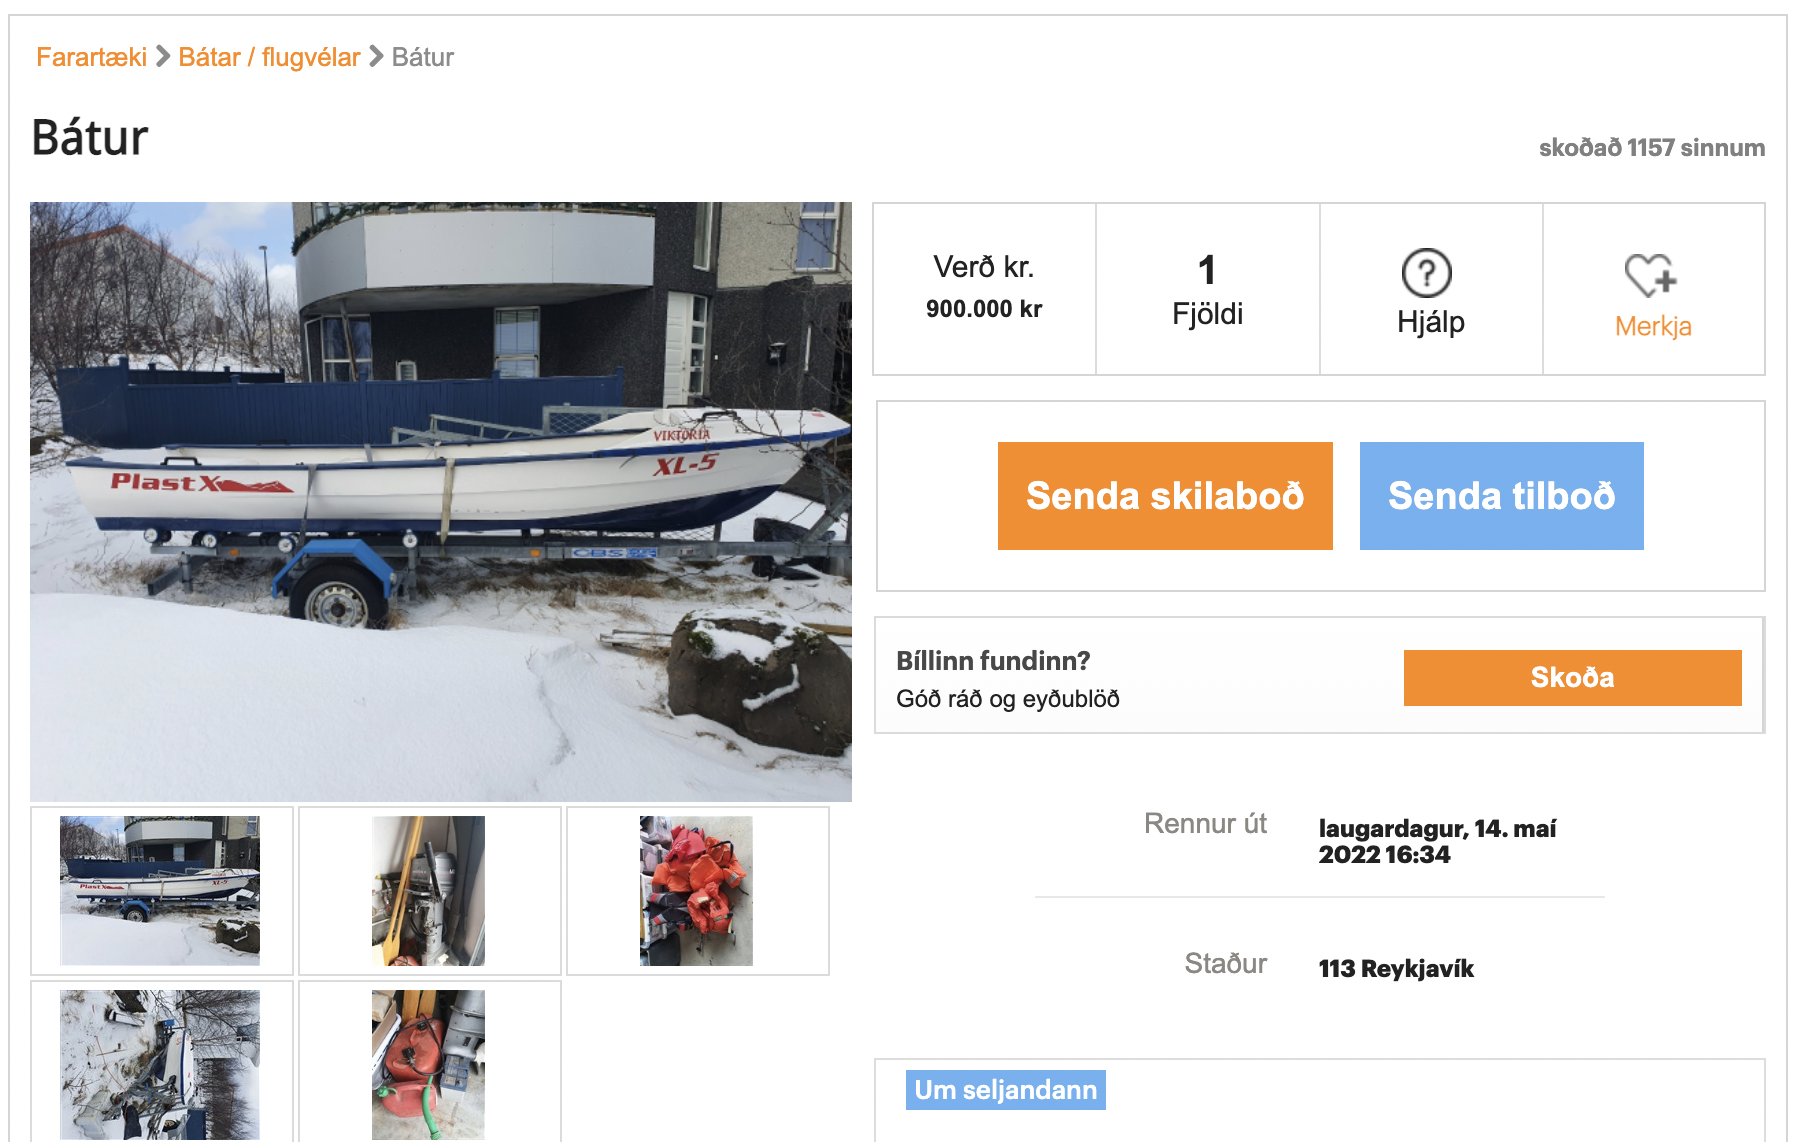
\includegraphics[width=150mm, height=80mm]{Images/benchmarking/product_page_bland.png}
\captionof{figure}{bland.is Product page}
    \end{center}
\end{Figure}
\begin{Figure}
    \begin{center}
        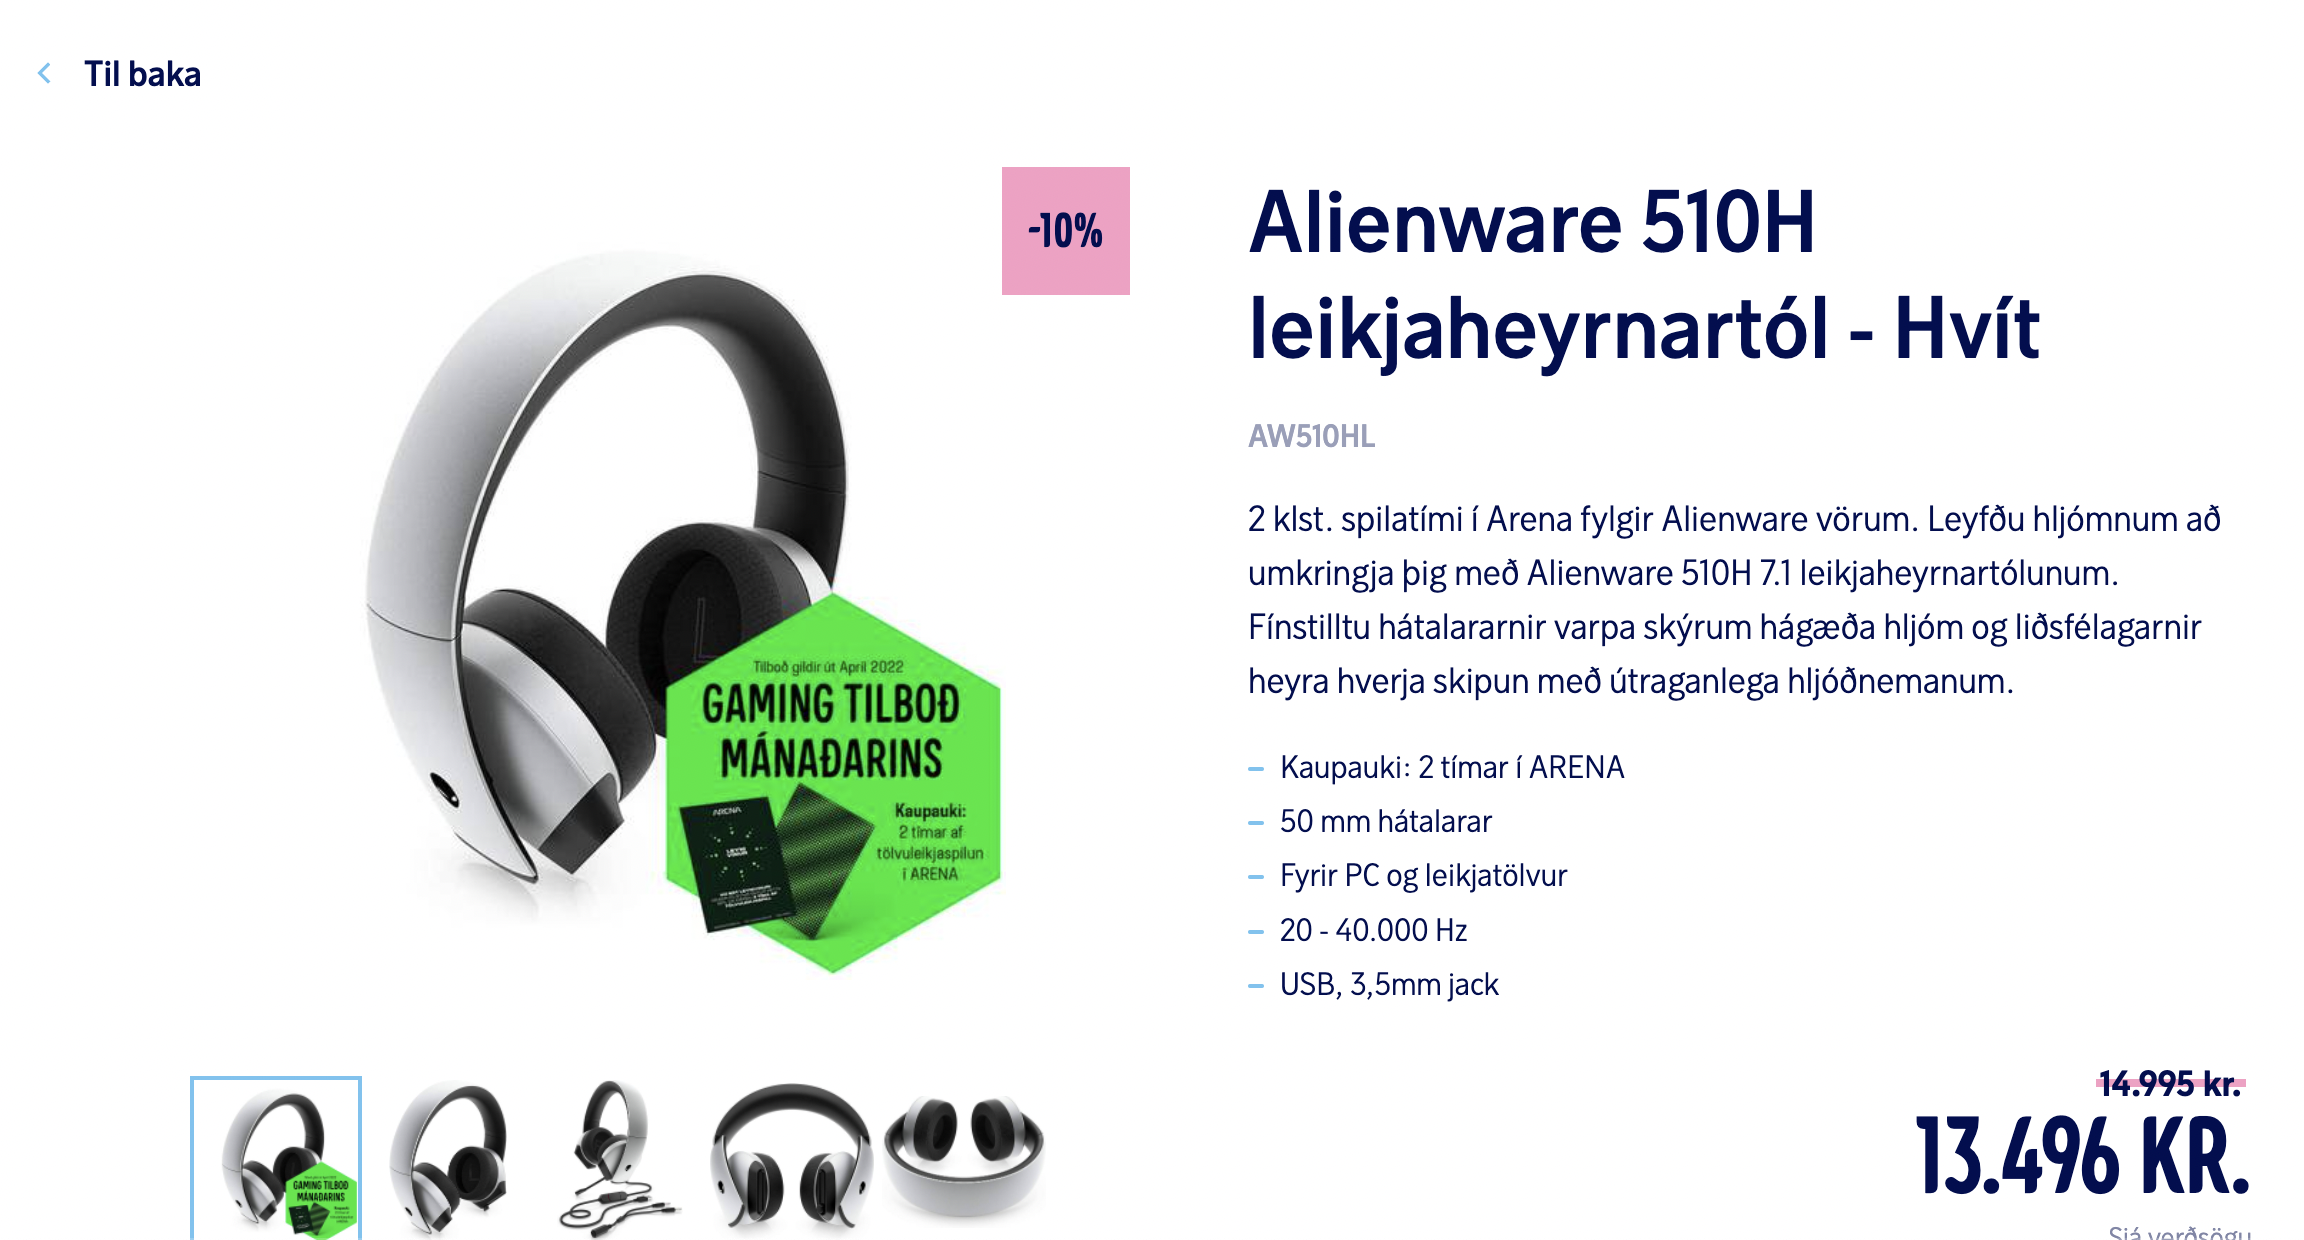
\includegraphics[width=150mm, height=80mm]{Images/benchmarking/product_page_elko.png}
\captionof{figure}{elko.is Product page}
    \end{center}
\end{Figure}
Omitted in the product page screenshot is the side and navigation bar, as we want to focus on the information on the product page.\\

Something that all these product pages have in common is the image gallery, Big emphasis is on the product images, and all but Elko put focus away from the item description. Craigslist, focusing on location and Bland focusing on doing an action. Elko has a small sale pitch with some key notes.\\

Viewing these screenshots in a small window, Elko has some nice features, that really show how they emphasise on the name of the product, an image and the price. All of these features, sans the image, are harder to make out in the other examples.

\subsection{Search results}
Search results give us what we want, hopefully. The play a key role in any data driven website and must be thought about carefully. 

As always, we base our benchmark on Craigslist and Bland, with the addition of Ebay. \textit{see figures 6, 7, 8}

\begin{Figure}
    \begin{center}
        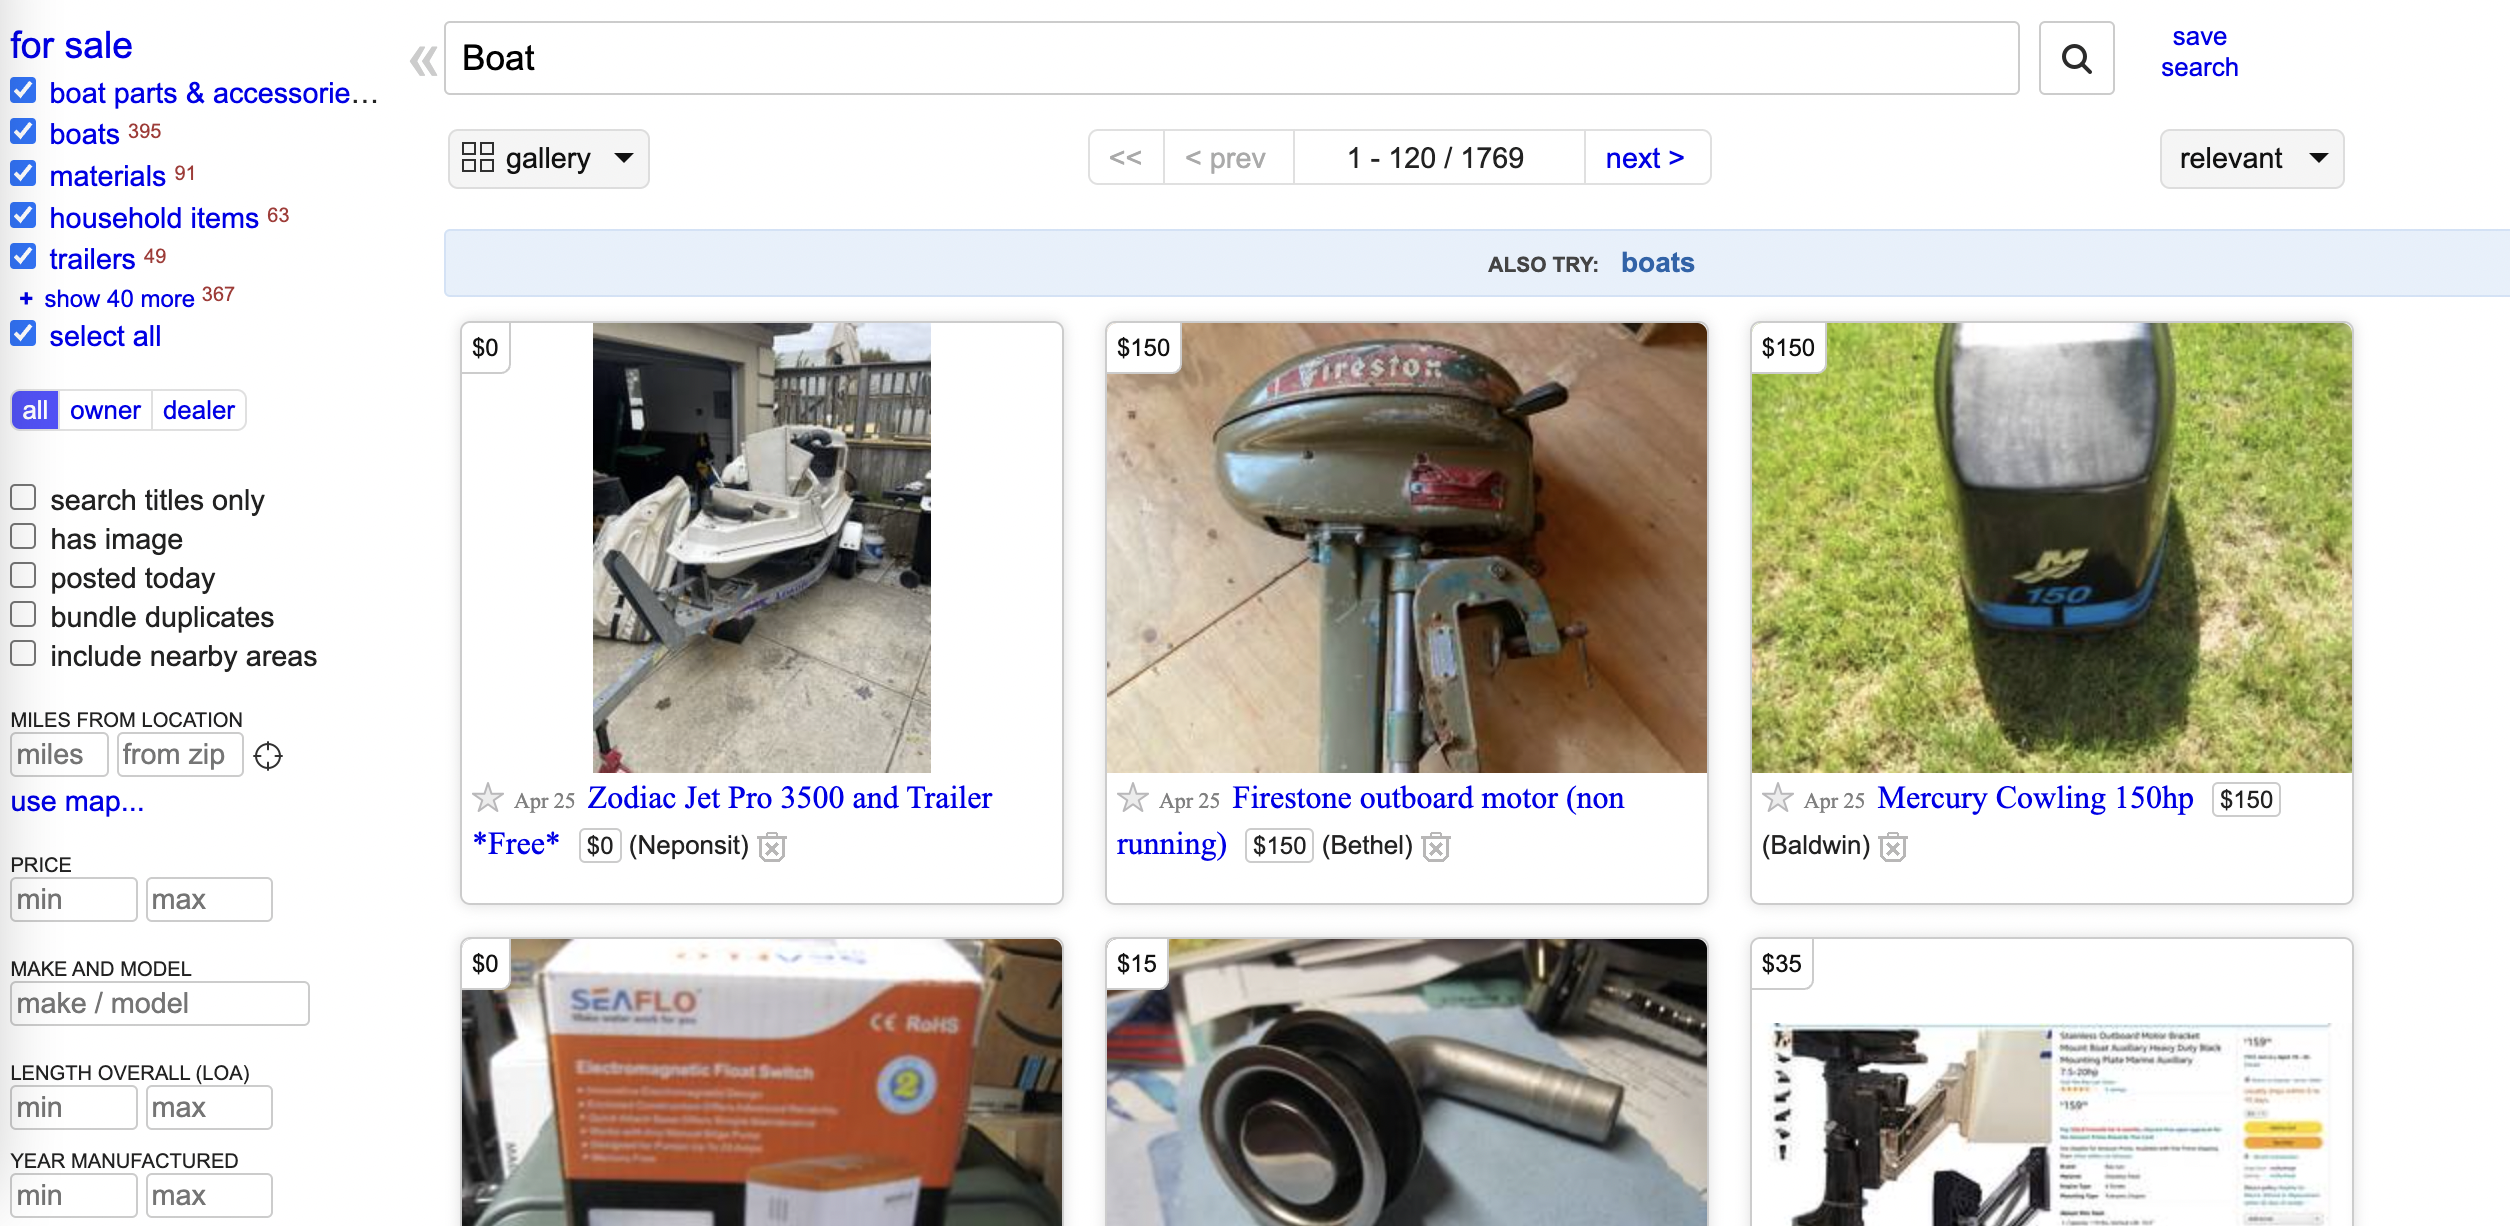
\includegraphics[width=150mm, height=80mm]{Images/benchmarking/search_result_cl.png}
\captionof{figure}{Craigslist search result page}
    \end{center}
\end{Figure}
\begin{Figure}
    \begin{center}
        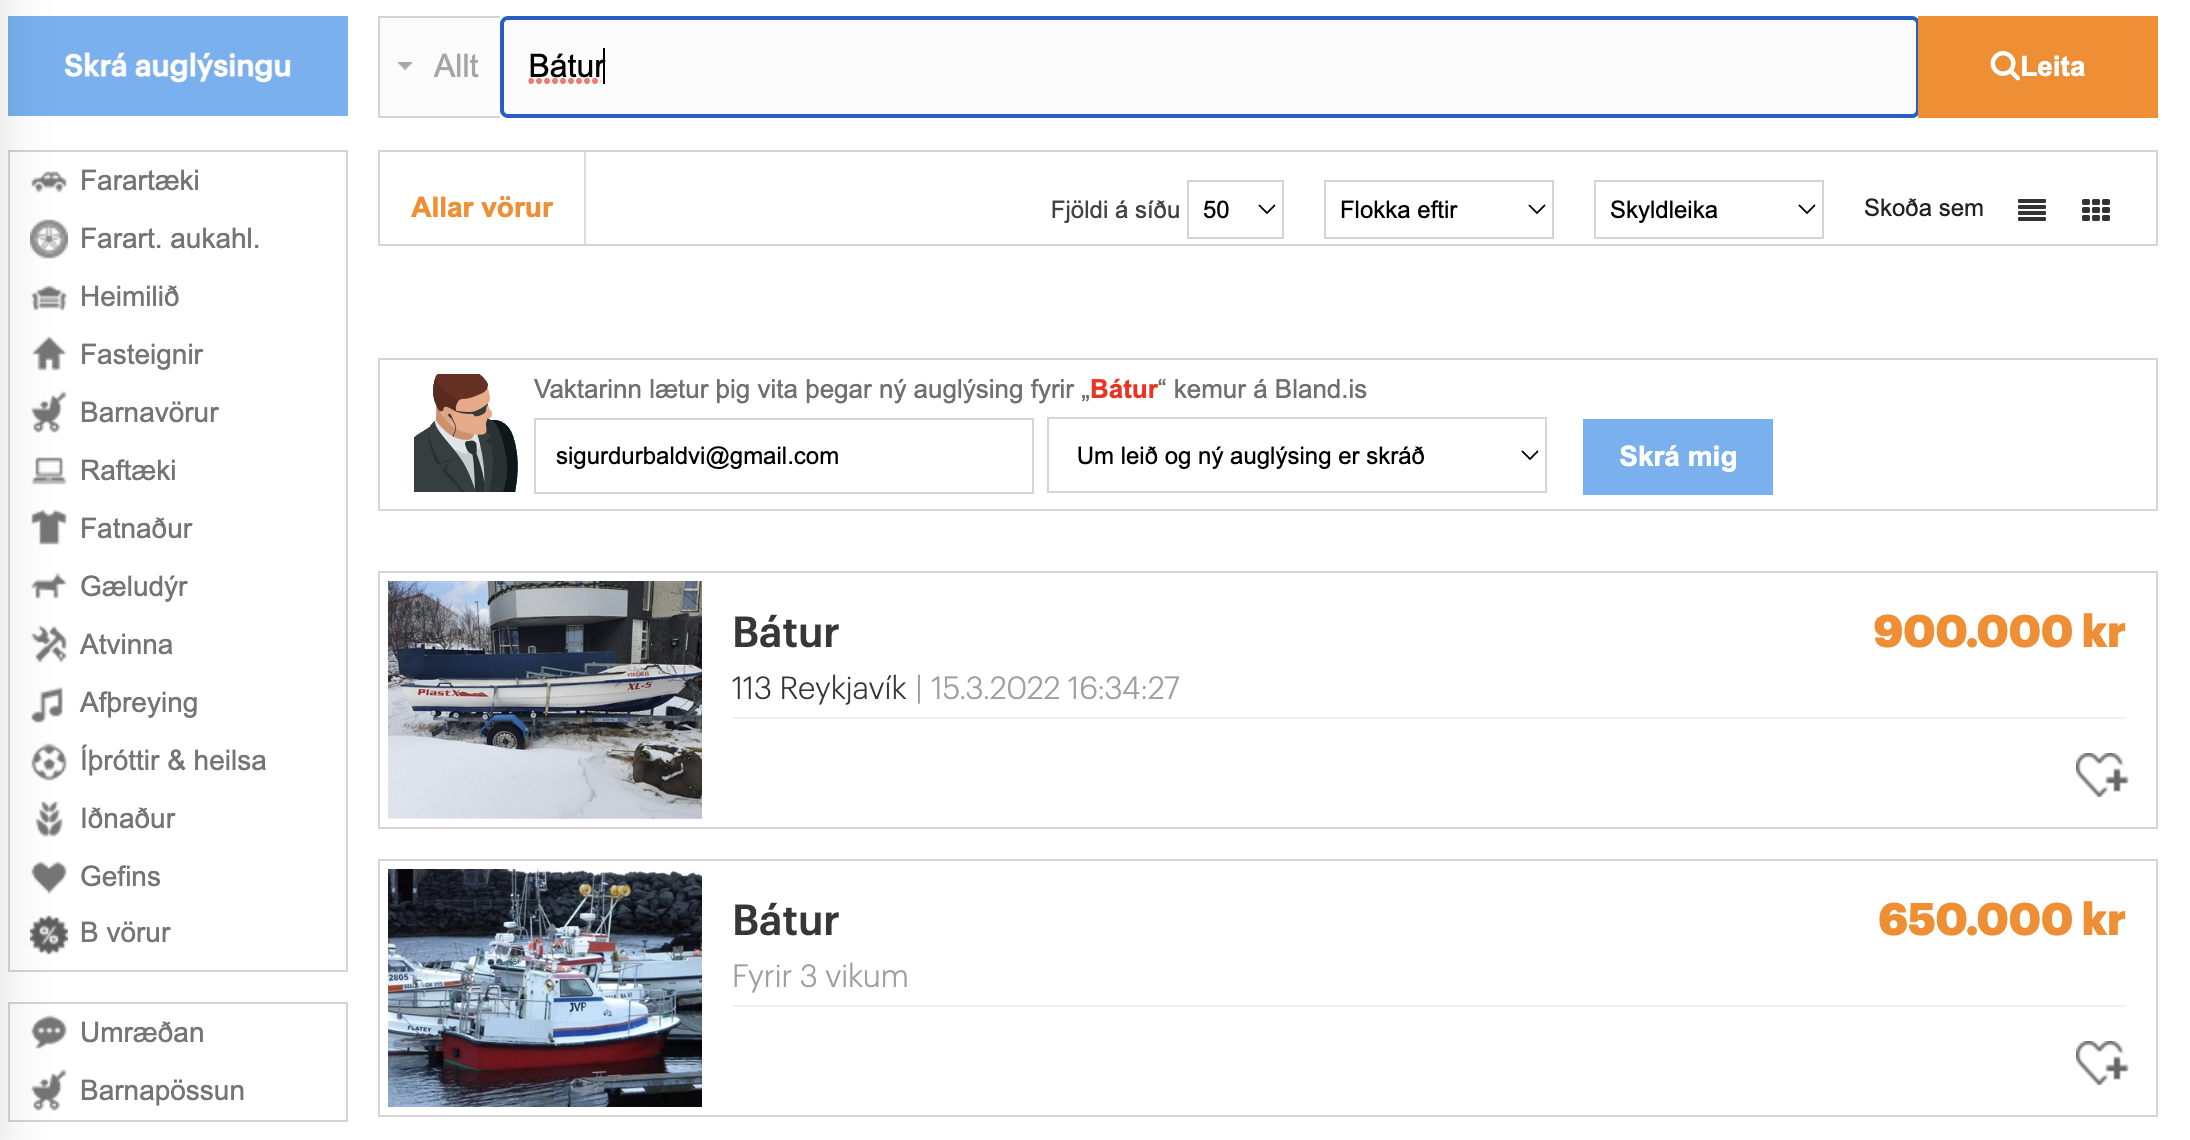
\includegraphics[width=150mm, height=80mm]{Images/benchmarking/search_result_bland.png}
\captionof{figure}{Bland.is search result page}
    \end{center}
\end{Figure}
\begin{Figure}
    \begin{center}
        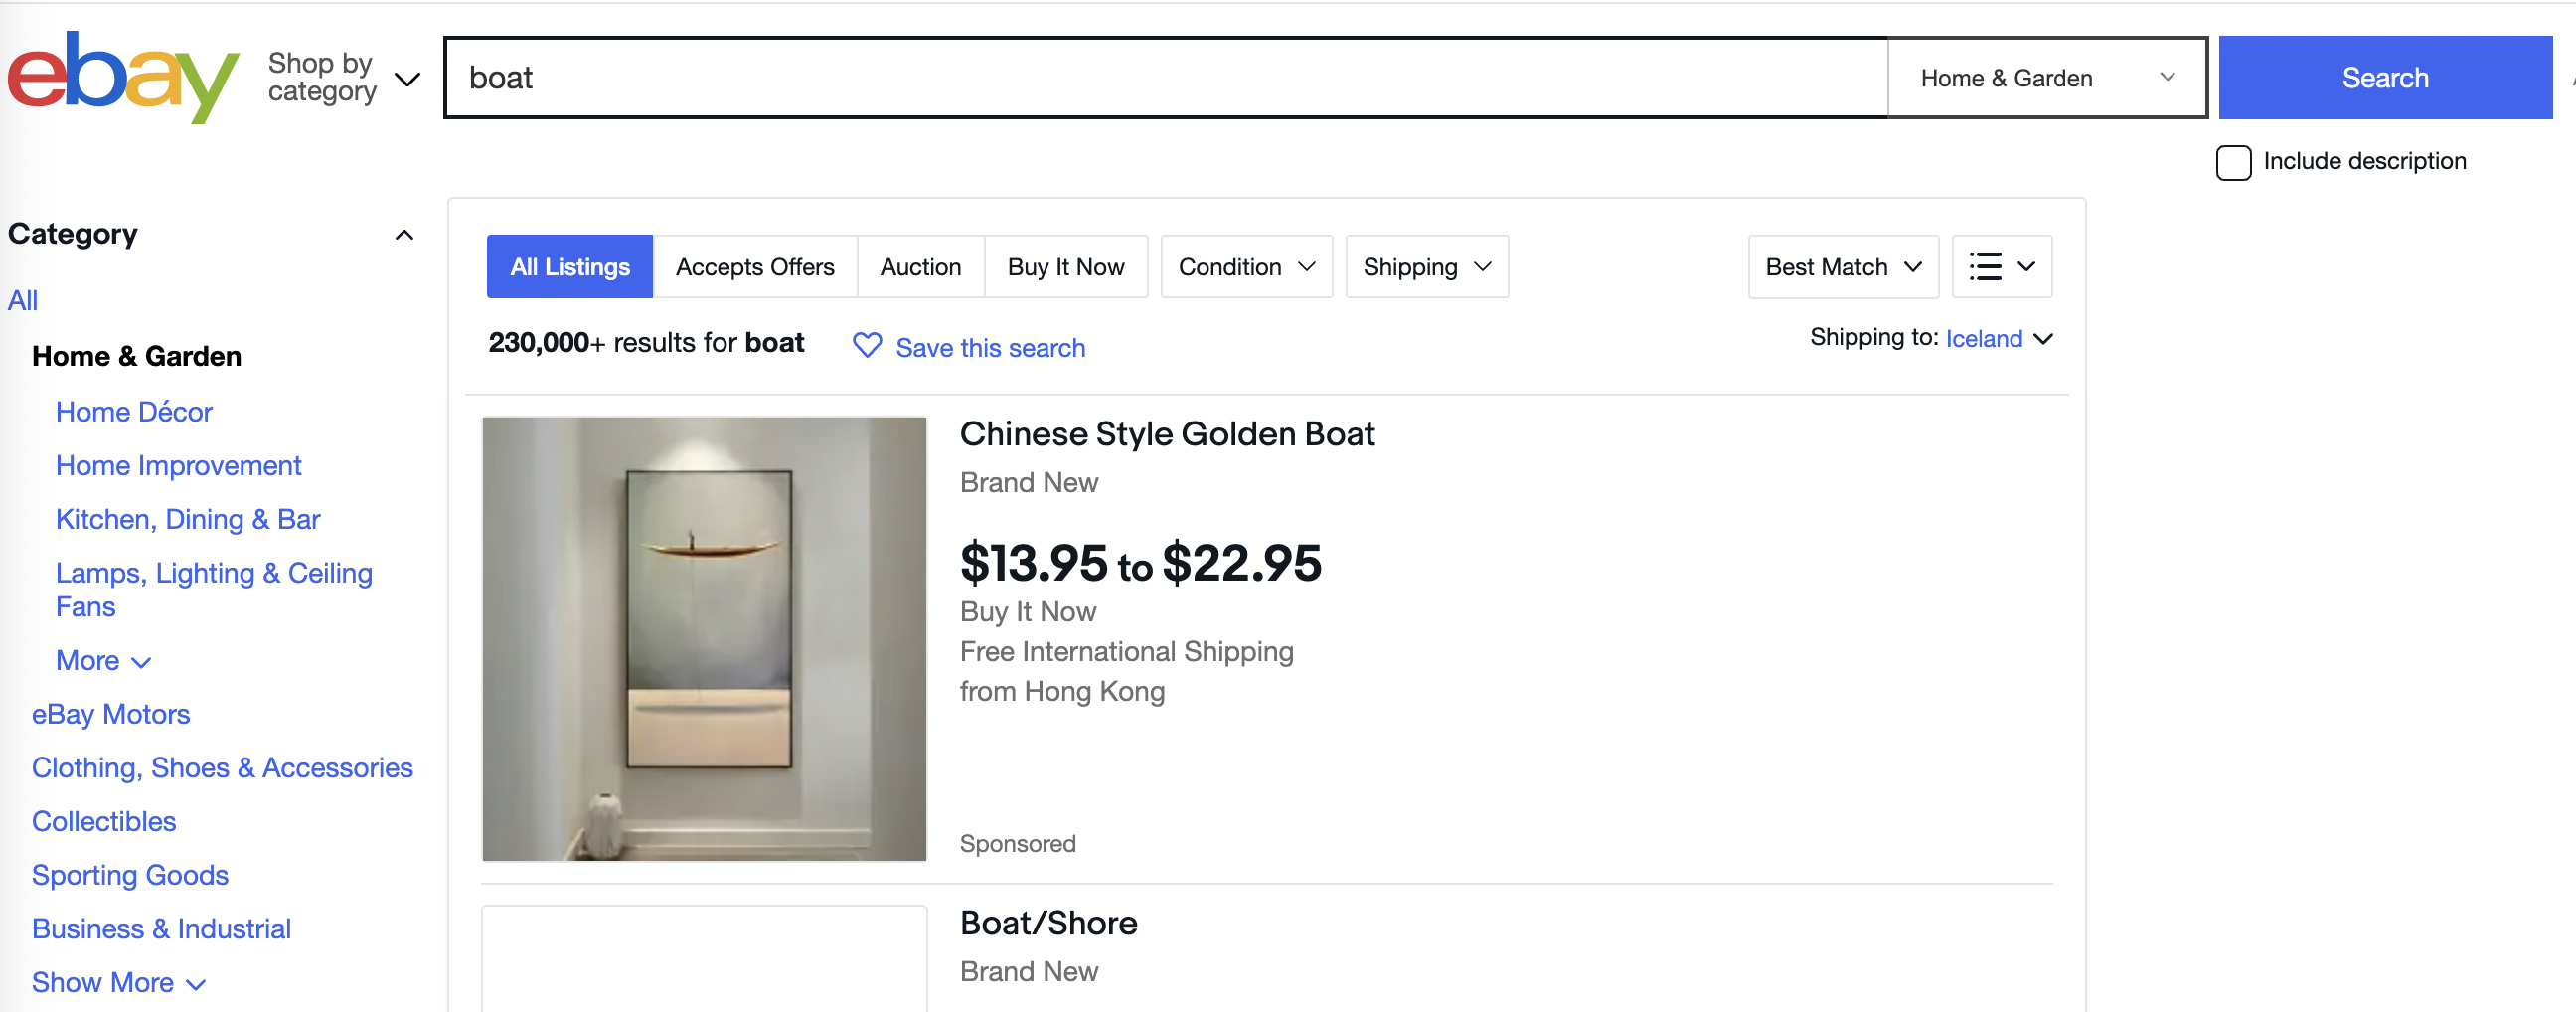
\includegraphics[width=150mm, height=80mm]{Images/benchmarking/search_result_ebay.png}
\captionof{figure}{Ebay's search result page}
    \end{center}
\end{Figure}
One of the metrics we can use is the number of visible search results, Craigslist being the "winner" in that category. Although the number of results might seem important, Bland and Ebay, in our opinion give better results, as they put their focus on the price, which is important to consumers in the used marketplace.\\

Bland in particular uses vibrant colors in their search result for prices, but opt for a black color and less emphasis when viewing the product page. Clearly expecting customers to be drawn into the product based on price from search results. Craigslist focuses on showing you the images of the product, letting that draw you in and never really focusing on the price. Ebays approach is also interesting as they give you only one result in the view but focusing on pricing, availability and the product information. 

\section{Conclution}

\section{Addendum}

\end{document}